%! Author = sbbfti
%! Date = 10/06/2020

%% Use the option review to obtain double line spacing
%% \documentclass[preprint,review,12pt]{elsarticle}

%% Use the options 1p,twocolumn; 3p; 3p,twocolumn; 5p; or 5p,twocolumn
%% for a journal layout:
%% \documentclass[final,1p,times]{elsarticle}
%% \documentclass[final,1p,times,twocolumn]{elsarticle}
%% \documentclass[final,3p,times]{elsarticle}
\documentclass[final,3p,times,twocolumn]{elsarticle}
%% \documentclass[final,5p,times]{elsarticle}
%% \documentclass[final,5p,times,twocolumn]{elsarticle}

%% \documentclass[review, 1p]{elsarticle}

\usepackage{mypreamble}
\usepackage{setspace}

\usepackage[nonumberlist,nogroupskip]{glossaries}

\newglossaryentry{7730}
{
name={ISO~7730:2005},
description={ISO~7730:2005 is a thermal comfort standard developed by ISO}
}

\newglossaryentry{55}
{
name={ASHRAE~55--2020},
description={ASHRAE~55--2020 is a thermal comfort standard developed by ANSI and ASHRAE}
}

\makenoidxglossaries


\begin{document}

    \begin{frontmatter}

    \title{Graph Attention Network (GAT) based Branching in
Combinatorial Optimization Problems}

    \author[label1]{Gökhan Murali\corref{mycorrespondingauthor}}
    \ead{gmurali21@ku.edu.tr}
    \author[label1]{Prof. Metin Türkay}

    \affiliation[label1]{organization={Koc University},
             addressline={Rumelifeneri Yolu, Sariyer},
             city={Istanbul},
             postcode={34450},
             %state={NSW},
             country={Turkiye}}

    \cortext[mycorrespondingauthor]{Corresponding author}

    \begin{abstract}


        In this study, the main aim is to imitate the Strong Branching strategy during the branching phase, which is one of the most critical components of the Branch \& Bound algorithm used for solving Combinatorial Optimization problems, by implementing a Graph Attention Network (GAT)-based method.
        Strong Branching is an effective strategy in terms of the number of nodes, keeping the search tree short.
        However, it is highly time consuming because it solves the linear programming problem twice for each branching candidate variable at each node.
        To eliminate the time cost of the Strong Branching strategy, this study attempts to learn a function implementing the GAT technique that can make Strong Branching-like decisions in a shorter time.

        In the literature, there are studies that successfully imitate the Strong Branching strategy using Graph Convolutional Neural Network (GCNN). In the GCNN method, all neighbouring nodes have the same importance for a node.
        In contrast, the GAT  architecture allows neighbouring nodes to have different levels of importance for a node.
        Therefore, it is hypothesized that GAT-based methods will yield better results.

        Experiments conducted in this study have shown that the GAT architecture provides decisions closer to the Strong Branching strategy compared to the GCNN architecture.
        GAT-based methods enable problems to be solved with fewer nodes compared to GCNN.
        In summary, GAT is a promising tool for imitating the effective yet slow Strong Branching strategy.
        Supplementary code for this study can be found at \url{https://github.com/GokhanMurali/learn2branchbyGAT}.
    \end{abstract}


    \begin{keyword}
        Mixed Integer Programming \sep Branch \& Bound \sep Strong Branching \sep Machine Learning \sep Neural Networks \sep Graph Neural Network (GNN) \sep Convolution \sep Message Passing \sep Graph Attention Network (GAT) \sep Graph Convolutional Neural Network (GCNN)
    \end{keyword}

\end{frontmatter}


    %%! Author = federico
%! Date = 10/06/2020

\section*{Nomenclature}
\renewcommand{\baselinestretch}{0.75}\normalsize
\renewcommand{\aclabelfont}[1]{\textsc{\acsfont{#1}}}
\begin{acronym}[longest]

    \acro{t-db}[$t_{db}$]{dry-bulb air temperature\acroextra{, $^{\circ}$C}}
    \acro{t-wb}[$t_{wb}$]{wet-bulb air temperature\acroextra{, $^{\circ}$C}}
    \acro{ti}[$t_{i}$]{indoor air temperature\acroextra{, $^{\circ}$C}}
    \acro{tout}[$t_{out}$]{outdoor air temperature\acroextra{, $^{\circ}$C}}
    \acro{t-op}[$t_{o}$]{operative air temperature\acroextra{, $^{\circ}$C}}
    \acro{t-cl}[$t_{cl}$]{clothing temperature\acroextra{, $^{\circ}$C}}
    \acro{tg}[$t_{g}$]{globe temperature\acroextra{, $^{\circ}$C}}
    \acro{rh}[$RH$]{relative humidity\acroextra{, \%}}
    \acro{v}[$V$]{average air speed\acroextra{, m/s}}
    \acro{t-r}[$\overline{t_{r}}$]{mean radiant temperature\acroextra{, $^{\circ}$C}}
    \acro{clo}[$I_{cl}$]{total clothing insulation\acroextra{, clo}}
    \acro{i-cl}[$i_{cl}$]{permeation efficiency of water vapor through the clothing layer}
    \acro{met}[$M$]{rate of metabolic heat production\acroextra{, W/m\textsuperscript{2}}}
    \acro{work}[$W$]{rate of mechanical work accomplished\acroextra{, W/m\textsuperscript{2}}}
    \acro{t-sk}[$t_{sk}$]{skin mean temperature\acroextra{, $^{\circ}$C}}
    \acro{t-sk-n}[$t_{sk,n}$]{neutral skin mean temperature\acroextra{, $^{\circ}$C}}
    \acro{t-cr}[$t_{cr}$]{core mean temperature\acroextra{, $^{\circ}$C}}
    \acro{t-re}[$t_{re}$]{rectal temperature\acroextra{, $^{\circ}$C}}
    \acro{t-cr-n}[$t_{cr,n}$]{neutral core mean temperature\acroextra{, $^{\circ}$C}}
    \acro{r-cl}[$R_{cl}$]{thermal resistance of clothing\acroextra{, m\textsuperscript{2}K/W}}
    \acro{r-e-cl}[$R_{e,cl}$]{evaporative heat transfer resistance of clothing layer\acroextra{, m\textsuperscript{2}kPa/W}}
    \acro{f-cl}[$f_{cl}$]{clothing area factor $A_{cl}/A_{body}$\acroextra{, m\textsuperscript{2}K/W}}
    \acro{h}[$h$]{sum of convective $h_{c}$ and radiative $h_{r}$ heat transfer coefficients\acroextra{, W/(m\textsuperscript{2}K)}}
    \acro{h-r}[$h_{r}$]{linear radiative heat transfer coefficient\acroextra{, W/(m\textsuperscript{2}K)}}
    \acro{h-c}[$h_{c}$]{convective heat transfer coefficient\acroextra{, W/(m\textsuperscript{2}K)}}
    \acro{h-e}[$h_{e}$]{evaporative heat transfer coefficient\acroextra{, W/(m\textsuperscript{2}kPa)}}
    \acro{a}[$\alpha$]{fraction of the total body mass considered
to be thermally in the skin compartment}

    \acro{cl-a}[$A_{cl}$]{clothing surface area\acroextra{, m\textsuperscript{2}}}

    \acro{e}[$\varepsilon$]{average emissivity of clothing or body surface}
    \acro{sigma}[$\sigma$]{Stefan-Boltzmann constant\acroextra{, 5.67 x 10\textsuperscript{-8} W/(m\textsuperscript{2}K\textsuperscript{2})}}

    \acro{a-r}[$A_{r}$]{effective  radiation  area  of  the  body\acroextra{, m\textsuperscript{2}}}
    \acro{body-a}[$A_{body}$]{body surface area\acroextra{, m\textsuperscript{2}}}
    \acro{body-w}[$mass$]{body mass\acroextra{, kg}}
    \acro{body-h}[$height$]{body height\acroextra{, m}}

    \acro{pmv}[PMV]{Predicted Mean Vote}
    \acro{ppd}[PPD]{Predicted Percentage of Dissatisfied\acroextra{, \%}}
    \acro{set}[SET]{Standard Effective Temperature\acroextra{, $^{\circ}$C}}
    \acro{ce}[CE]{Cooling Effect\acroextra{, $^{\circ}$C}}
    \acro{phs}[PHS]{Predicted Heat Strain}

    \acro{BMS}[BMS]{Building Management System}
    \acro{HVAC}[HVAC]{Heating, Ventilation, and Air Conditioning}
    \acro{VAV}[VAV]{Variable Air Volume}
    \acro{AHU}[AHU]{Air Handling Unit}

    \acro{ema}[EMA]{Ecological Momentary Assessment}
    \acro{sdk}[SDK]{Software Development Kit}
    \acro{api}[API]{Application Programming Interface}

    \acro{s-cr}[$S_{cr}$]{rate of heat storage in the core compartment\acroextra{, W/m\textsuperscript{2}}}
    \acro{s-sk}[$S_{sk}$]{rate of heat storage in the skin compartment\acroextra{, W/m\textsuperscript{2}}}
    \acro{s}[$S$]{rate of heat storage in the human body\acroextra{, W/m\textsuperscript{2}}}
    \acro{e-res}[$E_{res}$]{rate of evaporative heat loss from respiration\acroextra{, W/m\textsuperscript{2}}}
    \acro{e-dif}[$E_{dif}$]{rate of evaporative heat loss from moisture diffused through the skin\acroextra{, W/m\textsuperscript{2}}}
    \acro{e-rsw}[$E_{rsw}$]{rate of evaporative heat loss from sweat evaporation\acroextra{, W/m\textsuperscript{2}}}
    \acro{e-sk}[$E_{sk}$]{total rate of evaporative heat loss from skin\acroextra{, W/m\textsuperscript{2}}}
    \acro{e-max}[$E_{max}$]{maximum rate of evaporative heat loss from skin\acroextra{, W/m\textsuperscript{2}}}
    \acro{c-res}[$C_{res}$]{rate of convective heat loss from respiration\acroextra{, W/m\textsuperscript{2}}}
    \acro{c-r}[$C + R$]{sensible heat loss from skin\acroextra{, W/m\textsuperscript{2}}}
    \acro{q-res}[$q_{res}$]{total rate of heat loss through respiration\acroextra{, W/m\textsuperscript{2}}}
    \acro{q-sk}[$q_{sk}$]{total rate of heat loss from skin\acroextra{, W/m\textsuperscript{2}}}
    \acro{w}[$w$]{skin wettedness}
    \acro{w-max}[$w_{max}$]{skin wettedness practical upper limit}
    \acro{m-sweat}[$m_{rsw}$]{rate at which regulatory sweat is generated\acroextra{, mL/h\textsuperscript{2}}}
    \acro{m-bl}[$m_{bl}$]{skin blood flow\acroextra{, L/(hm\textsuperscript{2})}}
    \acro{c-sw}[$c_{sw}$]{driving coefficient for regulatory sweating\acroextra{, g/(hKm\textsuperscript{2})}}

    \acro{p-sk}[$p_{sk,s}$]{water vapor pressure at skin\acroextra{, kPa}}
    \acro{p-a}[$p_{a}$]{water vapor pressure in ambient air\acroextra{, kPa}}

    \acro{wmo}[WMO]{World Meteorological Organization}
    \acro{who}[WHO]{World Health Organization}
    \acro{cdc}[CDC]{Centers for Disease Control and Prevention}
    \acro{noaa}[NOAA]{National Oceanic and Atmospheric Administration}
    \acro{epa}[EPA]{United States Environmental Protection Agency}
    \acro{iea}[IEA]{International Energy Agency}
    \acro{un}[UN]{United Nations}

\end{acronym}
\renewcommand{\baselinestretch}{1}\normalsize


    %\doublespacing

    %% The lineno packages adds line numbers. Start line numbering with
    %% \begin{linenumbers}, end it with \end{linenumbers}. Or switch it on
    %% for the whole article with \linenumbers.
    %% \usepackage{lineno}

    \linenumbers

    \acresetall

    \section{Introduction}\label{sec:introduction}

If you are new to \LaTeX{}, you can check my YouTube video \href{https://youtu.be/CjuYkcA35dw}{\LaTeX{} Masterclass}.

If you are in a hurry, you can check my YouTube video \href{https://youtu.be/g0YdIs4oJm8}{Introduction to \LaTeX{}}.

\subsection{How to cite a paper}\label{subsec:how-to-cite-a-paper}
This is an example on how to cite a paper~\cite{Tartarini2020a}.

\subsection{How to add acronyms/nomenclature}\label{subsec:how-to-add-acronyms}
This is an example on how to add acronyms.
You can reference the acronym using the command \verb!\ac{t-db}! this will result in the following \ac{t-db}.
If you use the command \verb!\ac{t-db}! again, it will result in \ac{t-db}.
You can check the list of acronyms in the \texttt{myacronyms.tex} file.

\subsection{Glossary}\label{subsec:glossary}

This is an example on how to add a glossary.
You can reference the glossary using the command \verb!\gls{7730}! this will result in the following \gls{7730}.
You can check the list of glossary terms in the \texttt{myglossary.tex} file.

\subsection{How to add a table}\label{subsec:how-to-add-a-table}
This is an example on how to add a table.
The table is shown in Table~\ref{tab:example}.

\begin{table}[htb!]
    \centering
    \begin{tabular}{|c|c|}
        \hline
        \textbf{Column 1} & \textbf{Column 2} \\
        \hline
        Row 1 & Value 1 \\
        Row 2 & Value 2 \\
        Row 3 & Value 3 \\
        \hline
    \end{tabular}
    \caption{This is an example table.}
    \label{tab:example}
\end{table}

\subsection{How to add a figure}\label{subsec:how-to-add-a-figure}
This is an example on how to add a figure.
The figure is shown in Figure~\ref{fig:example}.

\begin{figure}[htb!]
    \centering
    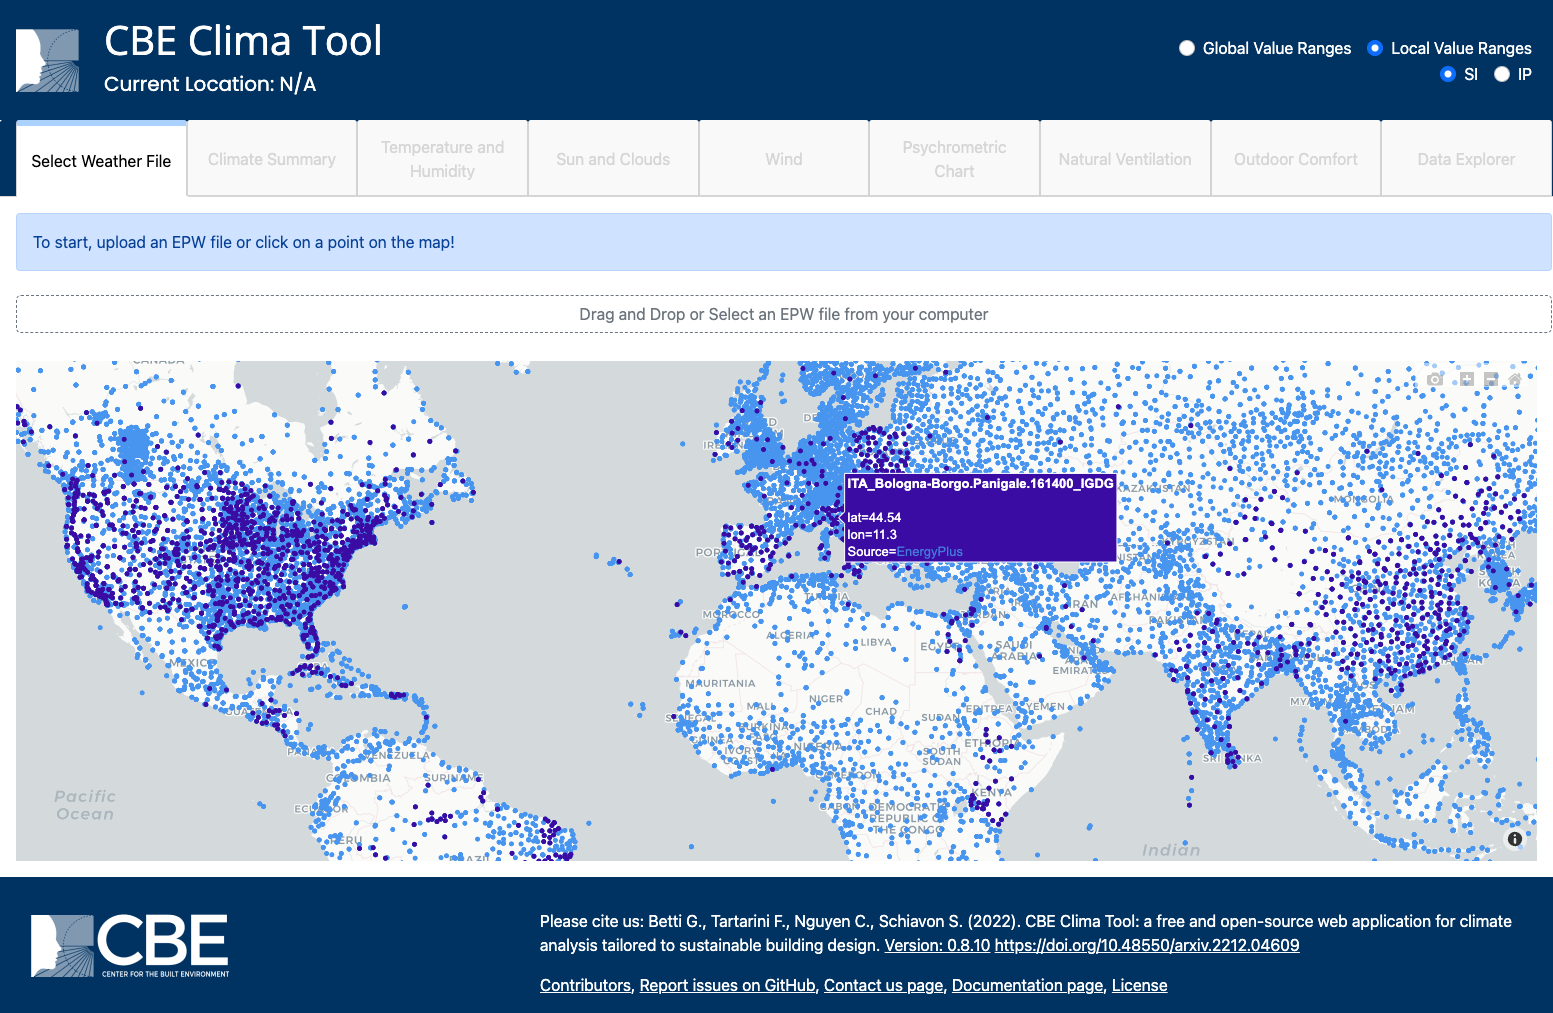
\includegraphics[width=0.75\textwidth]{figures/example_clima}
    \caption{This is an example figure.}
    \label{fig:example}
\end{figure}

\subsection{How to write numbers}\label{subsec:how-to-write-numbers}
This is an example on how to write numbers.

\subsection{How to import a variable}\label{subsec:how-to-import-a-variable}
This is an example on how to import a variable.
You can import a variable using the command \verb!\var{example_variable}! this will result in the following \var{example_variable}.
You can check the list of variables in the \texttt{mydata.tex} file.
If you want to find out more on how to import variables, you can check my YouTube video \href{https://ctan.org/pkg/datatool}{datatool} package documentation.

    \section{Background}\label{sec:background}

\subsection{Mixed Integer Linear Programming (MILP) Problems}\label{subsec:mixed-integer-linear-programming-(milp)-problems}


These problems are linear optimization problems where some of the decision variables are integers, and some are continuous.
It is possible to formulate MILP problems as follows:

\begin{equation}
    \begin{aligned}
        \text{minimize} \quad & \textbf{c}^T \textbf{x} \\
        \text{s.t.} \quad & \textbf{A}\textbf{x} \leq \textbf{b} \\
        & \textbf{x} \in \mathbb{Z}^p \times \mathbb{R}^{n-p}\\
    \end{aligned}\label{eq:equation}
\end{equation}


where \textbf{c} \begin{math} \in \mathbb{R}^n \end{math} represents the objective coefficient vector, \textbf{A} \begin{math} \in \mathbb{R}^{mxn} \end{math} represents the constraint coefficient matrix,  represents the right-hand-side vector, and  p \begin{math} \leq \end{math} n indicates the number of integer variables.
MILP problems are usually solved by Branch \& Bound algorithm.


\subsection{The LP Relaxation of a MILP Problem}\label{subsec:the-lp-relaxation-of-a-milp-problem}


LP Relaxation of a MILP problem is the problem obtained by ignoring the integrality conditions on the variables in the MILP problem as follows:

\begin{equation}
    \begin{aligned}
        \text{minimize} \quad & \textbf{c}^T \textbf{x} \\
        \text{s.t.} \quad & \textbf{A}\textbf{x} \leq \textbf{b} \\
        & \textbf{x} \in \mathbb{R}^{n}\\
    \end{aligned}\label{eq:equation}
\end{equation}


It is possible to solve this form of the problem using Linear Programming (LP) techniques such as Simplex algorithm.


\subsection{Bipartite Graph Representation of a MILP Problem}
\label{sec:bipartite_graph_representation}


To employ GNN techniques, such as GCNN and GAT, in tackling Combinatorial Optimization problems, these problems need to be represented as graphs.
Combinatorial Optimization problems can be represented as bipartite graphs.
The nodes on the left side of the bipartite graph represent the constraints in the MILP problem, with each constraint corresponding to a node.
The nodes on the right side of the bipartite graph represent the variables in the MILP problem, with each variable corresponding to a node.
If a variable is part of a constraint, there is an undirected edge between the corresponding nodes.
The coefficient of the variable in the constraint is a feature of the corresponding edge.
Figure 2.1 illustrates the bipartite graph representation of a MILP problem with 3 variables and 2 constraints.

This is an example on how to add a figure.
The figure is shown in Figure~\ref{fig:biparite-graph}.

\begin{figure}[htb!]
    \centering
    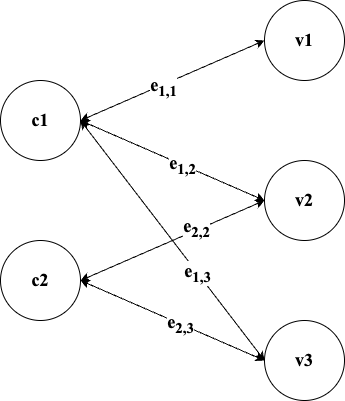
\includegraphics[width=0.45\textwidth]{figures/Bipartite Graph.drawio}
    \caption{Bipartite graph representation of a MILP problem with n = 3 variables and m = 2 constraints. If a variable is part of a constraint, there is an undirected edge between the corresponding nodes.}
    \label{fig:biparite-graph}
\end{figure}

    \section{Related Work}\label{sec:relatedWork}

Strong Branching is an efficient branching strategy in terms of the number of nodes generated but is costly in terms of time.
To mitigate the time cost disadvantage of the Strong Branching strategy, researchers have focused on developing strategies that can make Strong Branching-like decisions more quickly and efficiently.
One group of researchers aimed to leverage machine learning techniques to learn a function that would mimic the Strong Branching strategy.


\subsection{ExtraTrees Based Imitation of Strong Branching}\label{subsec:extratrees-based-imitation-of-strong-branching}
One of the pioneering studies in this field belongs to Alvarez et al.~\cite{alvarezMachineLearningBasedApproximation2017}.
In this study, Alvarez et al.~\cite{alvarezMachineLearningBasedApproximation2017} attempted to mimic the Strong Branching strategy by using a machine learning algorithm called ExtraTrees~\cite{geurtsExtremelyRandomizedTrees2006}.
The method used in this study consists of three steps.


In first step, randomly generated set covering (SC), multi knapsack (MKN), bin packing (BP), and equality (EQ) problems were solved using the Strong Branching strategy.
In addition to the Strong Branching scores calculated for each variable at each node, static problem features such as cost coefficient of variable $i$, dynamic problem features such as the fractionality of variable $i$ at the current solution and dynamic optimization features such as the number of times variable $i$ has been chosen as branching variable were also recorded for use during the training phase.
Detailed description of features can be seen in Appendix A Table 0.1. % burası revize edilecek


In second step, a function to mimic Strong Branching was learned using the ExtraTrees machine learning algorithm with $10^5$ training examples.
Alvarez et al.~\cite{alvarezMachineLearningBasedApproximation2017} approached the problem as a regression problem.
The recorded features were utilized as inputs to learn a weight vector for calculating the Strong Branching score for each branching candidate variable, in a manner similar to the Strong Branching strategy.
It can be stated that the learning process occurs offline.


In third step, the learned heuristic and other branching strategies (Random Branching, Most Infeasible Branching (MIB), Nonchimerical Branching (NCB), Full Strong Branching (FSB), and Reliability Branching (RB) were tested on two different datasets: randomly generated problems and standard benchmark problems from MIPLIB.
At this stage, two types of experiments were performed.
The first involved terminating the optimization process early, based on a predefined limit on either the number of nodes(a limit of $10^5$ nodes) explored or the computation time (a limit of 10 minutes) elapsed.
The second set of experiments allowed the problems to be solved to optimality, regardless of the time or node required.


An analysis of the experimental results, where MIPLIB problems were solved using CPLEX under node and time limits, reveals that the proposed branching strategy performs comparably to strong branching in both scenarios.
However, the performance of the learned branching strategy remains slightly inferior to that achieved with Reliability Branching (RB).
The closed gap (“Cl. Gap”) in Table~\ref{tab:alvarez-results} is defined as the ratio of the difference between the current dual bound and the objective value of the initial LP relaxation to the difference between the optimal objective value and the objective value of the initial LP relaxation.
A value close to 1 indicates that the optimization process is nearing its final stages.

\begin{table}[htb!]
    \centering
    \begin{tabular}{|c c c c c|}
        \hline
        \textbf{Criteria} & \textbf{S/T} & \textbf{Cl. Gap} & \textbf{Nodes} & \textbf{Time (s)}\\
        \hline
        \textbf{Node Limit} & & & & \\
        \textbf{Random} & 0/44 & 0.43 & 10,000 & 124.50 \\
        \textbf{MIB} & 6/44 & 0.50 & 9,274 & 233.19 \\
        \textbf{NCB} & 11/44 & 0.72 & 7,322 & 232.74\\
        \textbf{FSB} & \textbf{12/44} & \textbf{0.73} & \textbf{7,184} & 629.87 \\
        \textbf{RB} & 10/44 & 0.64 & 7,806 & 219.39 \\
        \textbf{Learned} & 10/44 & 0.62 & 8,073 & \textbf{162.87}\\
        \hline
        \textbf{Time Limit} & & & & \\
        \textbf{Random} & 0/44 & 0.47 & 867,837 & 600.01 \\
        \textbf{MIB} & 3/44 & 0.52 & 764,439 & 561.27\\
        \textbf{NCB} & 5/44 & \textbf{0.73} & 101,408 & 513.00 \\
        \textbf{FSB} & 3/44 & 0.66 & \textbf{49,008} & 534.65 \\
        \textbf{RB} & \textbf{7/44} & 0.69 & 257,375 & 515.40\\
        \textbf{Learned} & 5/44 & 0.63 & 130,081 & \textbf{512.72} \\
        \hline
    \end{tabular}
    \caption{Optimization results under node and time limits on MIBLIP dataset for different branching strategies.
    The best value is in bold.
    “S/T” represents the ratio of problems solved within the given node or time limit to the total number of problems.}
    \label{tab:alvarez-results}
\end{table}


When we examine the experimental results in which MIPLIB problems were solved by CPLEX until optimality, as can be seen in Table~\ref{tab:alvarez-results-2}, it is observed that the learned function is the strategy that produces the fastest solutions when cuts and heuristics are used by CPLEX.
It was observed that the learned function solved the problems with fewer nodes compared to the Random and MIB strategies.
However, in terms of node count, the learned function is less effective than the RB and NCB strategies.
When cuts and heuristics are not used by CPLEX learned function seems to be non-efficient in terms of node count and time.

\begin{table}[htb!]
    \centering
    \begin{tabular}{|c c c c c|}
        \hline
        \textbf{} & \multicolumn{2}{c}{\textbf{w/o cuts \& heuristics}} & \multicolumn{2}{c|}{\textbf{cuts \& heuristics}}\\
        \hline
        \textbf{Strategy} & \textbf{Nodes} & \textbf{Time(s)} & \textbf{Nodes} & \textbf{Time(s)} \\
        \hline
        \textbf{Random} & 7,809,341 & 29,377.10 & 152,564 & 503.38 \\
        \textbf{MIB} & 3,472,431 & 7,387.09 & 105,692 & 356.52 \\
        \textbf{NCB} & 145,244 & 1,136.34 & 34,500 & 1,451.74\\
        \textbf{FSB} & \textbf{129,047} & 1,597.12 & \textbf{25,941} & 895.36\\
        \textbf{RB} & 318,384 & \textbf{886.12} & 51,913 & 2,836.93\\
        \textbf{Learned} & 1,037,055 & 3,023.4 & 57,652 & \textbf{124.94}\\
        \hline
    \end{tabular}
    \caption{Optimization results (until termination) on MIBLIP dataset for different branching strategies.
    Lower is better, and the best value is in bold.}
    \label{tab:alvarez-results-2}
\end{table}


\subsection{ExtraTrees Based Imitation of Strong Branching}
Another study in this field was conducted by Khalil et al~\cite{khalilLearningBranchMixed2016}.
In this study, the researchers attempted to mimic the Strong Branching strategy using the svmRank machine learning algorithm.
This study consists of three steps.


In first step, unlike the study by Alvarez et al.~\cite{alvarezMachineLearningBasedApproximation2017}, in this research, training and testing were conducted on the same problem instance.
It can be stated that the learning process occurs online.
Branching was performed using Strong Branching for the first $\Theta$ nodes of each problem.
Each variable was assigned a label based on the Strong Branching score.
The following formula was used for label assignment:

\[ y_i^n = \begin{cases}
      1 & S_i^n\geq (1-\alpha)S_*^n \\
      0 & otherwise
   \end{cases}
\]

where $S_*^n$ is maximum SB score and the parameter $\alpha$ $\in$ [0, 1] represents the fraction of the maximum Strong Branching ($S_*^n$) that a variable must achieve to be assigned a label of '1'.
At each node, the assigned labels and the static features such as objective function coefficients and dynamic features such as the fractionality of variable i at the current solution were recorded as training data.
Detailed description of features can be seen in Appendix A Table 0.2. % burası revize edilecek


In second step, unlike Alvarez et al.~\cite{alvarezMachineLearningBasedApproximation2017}, Khalil et al.~\cite{khalilLearningBranchMixed2016} approached the problem as a ranking problem.
Instead of predicting the Strong Branching score as Alvarez et al.~\cite{alvarezMachineLearningBasedApproximation2017} did, the researchers focused on ranking the variables among themselves in a manner similar to Strong Branching.
According to the researchers, the exact Strong Branching score is not important; what matters is that the variables are ranked among themselves in the way Strong Branching would.
At this stage, a linear function ($f$) was learned using the svmRank~\cite{joachimsTrainingLinearSVMs2006} machine learning algorithm and Pairwise loss~\cite{joachimsOptimizingSearchEngines}:

\[
f: \mathbb{R}^p \rightarrow \mathbb{R}, \quad
f\left(\Phi(x_i, N_n)\right) = \mathbf{w}^T \Phi(x_i, N_n), \quad
\]

\[
\hat{y}_i^n = f\left(\Phi(x_i, N_n)\right)
\]

\[
\mathbf{w}^* = \arg\min_{\mathbf{w} \in \mathbb{R}^p}
\sum_{N_n \in N} \ell(\mathbf{y}^n, \hat{\mathbf{y}}^n)
+ \lambda \| \mathbf{w} \|_2^2
\]

where $\Phi(x_i, N_n)$ denotes variable $x_i$ at node $N_n$ with $p$ features, $\mathbf{w}^*$ denotes learned weight vector, $\ell$ denotes the loss function (Pairwise loss), $\lambda$ denotes regularization parameter that helps to avoid overfitting, $\hat{\mathbf{y}}^n$ denotes vector of values resulting from applying $f$ to every fractional variable in $N_n$, $\mathbf{y}^n$ denotes the true label of every fractional variable in $N_n$.


In third step, the learned weight vector was used for branching instead of Strong Branching.
The feature vectors of the variables were multiplied by the learned weight vector to calculate a score for each variable.
The variable with the highest score was selected for branching.


In the experimental phase, the developed method (SB+ML) was tested on MIPLIB2010 problems.
The results were compared with CPLEX's default branching strategy (CPLEX-D), Strong Branching (SB), Pseudocost Branching (PC), and the SB + PC strategy. SB+PC is a hybrid approach that uses SB for the first $\Theta$ = 500 nodes, and PC afterward.
Experiments were conducted on a total of 523 problems.
Problems solved by CPLEX-D with fewer than 50,000 nodes were classified as Easy, those solved with more than 50,000 but fewer than 500,000 nodes as Medium, and those solved with more than 500,000 nodes as Hard.
The experimental results are summarized in the Table~\ref{tab:khalil-results}:

\begin{table}[ht]
\centering
\small
\begin{tabular}{|lcccccc|}
\toprule
 & \textbf{CPLEX-D} & \textbf{SB} & \textbf{PC} & \textbf{SB+PC} & \textbf{SB+ML} \\
\midrule
\textbf{Unsolved} & & & & & \\
\textbf{Instances} & & & & & \\
\quad All (523) & 11 & 129 & 66 & 63 & \textbf{52} \\
\quad Easy (255) & 0 & 12 & 15 & 14 & \textbf{13} \\
\quad Medium (120) & 2 & 43 & 22 & 22 & \textbf{17} \\
\quad Hard (148) & 9 & 74 & 29 & 27 & \textbf{22} \\
\midrule
\textbf{Number of} & & & & & \\
\textbf{Nodes} & & & & & \\
\quad All (523) & 46,633 & 33,072 & 92,662 & 70,455 & \textbf{59,223} \\
\quad Easy (255) & 3,255 & 3,610 & 7,931 & 5,224 & \textbf{5,124} \\
\quad Medium (120) & 173,417 & 121,923 & 395,199 & 288,916 & \textbf{234,093} \\
\quad Hard (148) & 1,570,891 & 519,878 & 1,971,333 & 1,979,660 & \textbf{1,314,263} \\
\midrule
\textbf{Total Time} & & & & & \\
\textbf{(s)} & & & & & \\
\quad All (523) & 499 & 2,263 & \textbf{960} & 1,093 & 1,059 \\
\quad Easy (255) & 111 & 602 & \textbf{243} & 361 & 382 \\
\quad Medium (120) & 1,123 & 6,169 & 2,493 & 1,892 & \textbf{1,776} \\
\quad Hard (148) & 3,421 & 9,803 & 4,705 & 4,718 & \textbf{4,039} \\
\bottomrule
\end{tabular}
\caption{“Unsolved instances” are counts, “Num. nodes” and “Total time” (in seconds) are shifted geometric means over instances with shifts 10 and 1, respectively.
Lower is better, and the best value in each row among PC, SB+PC and SB+ML is in bold.}
    \label{tab:khalil-results}
\end{table}


The researchers analyzed the experimental results from three perspectives: the number of unsolved problems, the total number of nodes, and the total solution time.
Since the researchers claimed that the developed method is better at selecting branching variables, the primary metric they focused on was the total number of nodes.
As can be seen from the table above, the developed method (SB+ML) is more successful in terms of the total number of nodes compared to PC and SB+PC.
When considering all the problems, it was observed that the developed method reduced the solution time compared to the Strong Branching strategy, while increasing the number of nodes.


\subsection{GCNN Based Imitation of Strong Branching}\label{subsec:gcnn-based-imitation-of-strong-branching}
In another study in this field, Gasse et al.~\cite{gasseExactCombinatorialOptimization2019} attempted to mimic the Strong Branching strategy using a Graph Convolutional Neural Network (GCNN).
In this study, the researchers used the bipartite graph representation of MILP problems, enabling the use of GCNN in solving MILP problems.
This study consists of three steps.


In first step, 100,000 branching examples were collected from 10,000 randomly generated MILP problems (Set Covering Problems, Combinatorial Auction Problems,Capacitated Facility Location Problems, Maximum Independent Set Problems).
For each branching example, the Strong Branching scores calculated for the variables and variable features such as objective coefficient, constraint features such as dual solution value, edge features such as constraint coefficient were collected.
Detailed description of features can be seen in Appendix A Table 0.3. % burası revize edilecek


In second step, unlike Alvarez et al.~\cite{alvarezMachineLearningBasedApproximation2017} and Khalil et al.~\cite{khalilLearningBranchMixed2016}, Gasse et al.~\cite{gasseExactCombinatorialOptimization2019} approached the problem as a classification problem.
They attempted to learn how to select the variable to be used in branching with a Graph Neural Network, mimicking the approach of the Strong Branching strategy.
The GNN architecture used here essentially consists of three components as can be seen in Figure 3.1.

    \section{Methodology}\label{sec:methodology}

    \section{Results}\label{sec:results}

    \section{Conclusions}\label{sec:conclusions}


    \clearpage

    \bibliography{mybibfile}

    \clearpage

    \appendix

\section{Appendix}\label{sec:appendix}


\end{document}